\section{Einleitung}%2-10

Diese Studienarbeit dokumentiert den Programmentwurf einer Party-Lichtsteuerung, vom Design der Anwendung über die Implementierung bis hin zur Bereitstellung einer lauffähigen Applikation.
Die Programmcode wird mit LabVIEW von National Instruments entwickelt.

\subsection{Aufgabenstellung}
Es ist ein Programm für Lichttechniker zu entwickeln, mit dem eine viel zahl von Scheinwerfer angesteuert werden kann. 
%Dabei soll ein durch den Lichttechniker erstellter Ablauf abgespielt werden.

\subsection{Anforderungen}
Der Light Jockey (LJ) stellt für verschiedene Lichtkanäle Intensität und Farbe ein. Für eine Gruppe von Lichkanälen (Set) kann eine Wartezeit, Überblendungszeit, Nachlaufzeit und Name eingestellt werden. Wählt der LJ die Schaltfläche zum aufnehmen, öffnet sich ein Fenster in dem die gewünschten Parameter übergeben werden. Nach der Bestätigung durch ein Klick auf die OK-Schaltfläche wird das erstellte Set hinten an die Queue angefügt.

Hat der Bediener einige Sets angelegt, wird mit der Abspiel-Schaltfläche das aufgenommene Programm durchlaufen. Ein Set das abgespielt wird wartet die angegebene Zeit, dann wird die Farbe bis zur Intensität über die Überblendungszeit hochgefahren. Jetzt beginnt die Nachlaufzeit, ist diese verstrichen wird mit dem nächsten Set aus der Queue fortgefahren. Der Bediener kann jeder Zeit eine abspielende Queue mit der Stopp-Schaltfläche anhalten.

Über die Menüleiste kann der Bediener mit dem Menüpunkt "`Datei"' die Queue speichern und laden. In beiden Fällen öffnet sich eine Dialogbox in dem nach Speicher- bzw. Ladepfad gefragt wird.

	\begin{figure}%[h!]
	\centering
		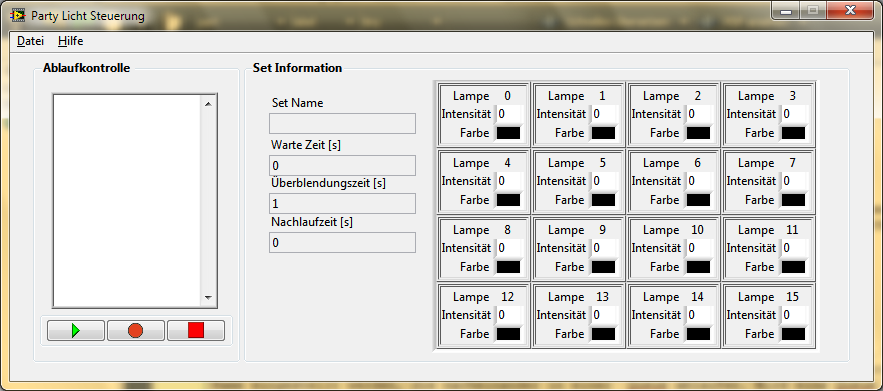
\includegraphics[width=\textwidth]{Pics/Oberflaeche001.png}
	\caption{Bedienoberfläche für die Party-Lichtsteuerung}
	\label{fig:ober001}
	\end{figure}



%\subsection{Motivation und Zielsetzung}

%Quelle: \cite{labview-buch01} \\
%Quelle: \cite{internet}
\subsection{Dokumentation}
Der LabVIEW Quellcode  sowie eine Ausführbare Windows-Anwendung mit der notwendigen RunTime als Insatller findet sich auf der beigelegten CD.
Auch enthalten sind die Programmcode ausschnitte als Bilder in hoher Detailansicht.
Und Projekt auf \url{http://code.google.com/p/party-licht-steuerung/}.


\subsection{Aufbau der Arbeit}

Bla Bla Blaaa




